% IFAC International Federation of Automatic Control paper template. 
% Created by: ?
% Modified by: Rasmus Christensen, Aalborg University, Denmark 15/12/2012
\documentclass{ifacconf}

\usepackage{natbib}            % you should have natbib.sty
\usepackage{graphicx}          % Include this line if your 
                               % document contains figures,
%\usepackage[dvips]{epsfig}    % or this line, depending on which
                               % you prefer.
\usepackage[utf8]{inputenc} % So we can input Nicks name in the paper title!
\usepackage[T1]{fontenc}
\usepackage{amsmath,amsfonts,amssymb} % Added so we can do pretty math equations.

% predefined environments
%\begin{thm} ... \end{thm}		% Theorem
%\begin{lem} ... \end{lem}		% Lemma
%\begin{claim} ... \end{claim}	% Claim
%\begin{conj} ... \end{conj}	% Conjecture
%\begin{cor} ... \end{cor}		% Corollary
%\begin{fact} ... \end{fact}	% Fact
%\begin{hypo} ... \end{hypo}	% Hypothesis
%\begin{prop} ... \end{prop}	% Proposition
%\begin{crit} ... \end{crit}	% Criterion


\begin{document}

\begin{frontmatter}

\title{Centralized State Estimation of Distributed Maritime Autonomous Surface Oceanographers\thanksref{footnoteinfo}} % Title, preferably not more than 10 words.

\thanks[footnoteinfo]{Thanks to the  has been paid for in full by the School of Information Communication and Technology.}

\author{Rasmus L. Christensen} 
\author{Frederik Juul} 
\author{Nick \O stergaard}
\author{Attila Fodor}
\author{Tudor Muresan}
\address{Department of Electronic Systems, Aalborg University, Fredrik Bajers Vej 7, 9220 Aalborg \O st, Denmark (e-mail: \{ralch,nickoe,fjuul,tmures12,afodor12\}@es.aau.dk)}                                            
          
\begin{keyword}                           % Five to ten keywords,  
Path planning; Centralised control; Baud rates; State estimation; Marine systems; Master slave system;              % chosen from the IFAC 
\end{keyword}                             % keyword list or with the 
                                          % help of the Automatica 
                                          % keyword wizard


\begin{abstract}                          % Abstract of not more than 250 words.
This paper considers the subject of running a centralized controller for the purpose of navigating a small Autonomous Surface Vehicle (ASV). The centralized controller is using a Kalman filter as a state predictor to improve the precision of the navigational aids mounted aboard. The work presents the design of the motion control system as well as the development of a protocol used to push through as much data on a standard 9.6 kbps data link simplex link.

The performance for the algorithms developed in this project, have been tested in Limfjorden in Aalborg, and towards the end, results of these tests are shown. 
\end{abstract}

\end{frontmatter}

\section{Introduction}
Seaborne measurements are often an expensive and time-consuming task. They could however in many cases have a large impact on the area where they are obtained. At the Fukushima accident in 2011 the area of effect in the water and the safety margin was primarily based on estimates, as only few measurements were available.
The coastal areas around Greenland are another area which could benefit from seaborne measurements as up to date maps are not available. This causes the ships which need to pass near the coast to have a higher safety margin, which in turn lowers the amounts of traffic possible. If a ship would need to get very close to the shores, up to date maps of the area would also be a requirement. This need is acknowledged and is considered important for the flourishing greenlandic industrialization by the government of Denmark, but the project does not have sufficient funding. \cite{engineer}.

One way to reduce the cost of such maritime measurements would be to develop small autonomous drones to carry out the task. These should be controlled by a mothership to enable easy scalability and coordination. Further, they should communicate using a simple data link to preserve bandwidth and limit power consumption. The system should be robust to dataloss and measurementnoise which can be expected from low cost sensors. This can be achieved through sensor fusion.

Currently the main focus of autonomous vehicles have been on aerial, ground and underwater vehicles, while there is close to no research going on about small autonomous surface vessels. An example of such a vessel is the Stingray ASV developed by Isreali Based Elbit Systems. The purpose of this vehicle is somewhat military related, while the purpose of measuring the coastal areas around Greenland are primarily humanitarian.
\begin{figure}
	\begin{center}
		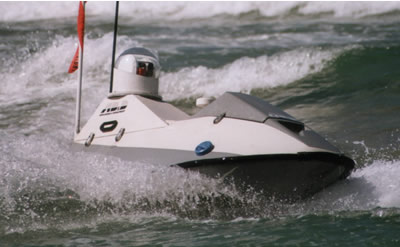
\includegraphics[width=8.4cm]{img/stingray.jpg} % width of a column is 8.4 cm.
		\caption{The autonomous surface vehicle Stingray by Israeli based Elbit Systems in action.}  
		\label{fig:stingray}
	\end{center}
\end{figure}

Figure \ref{fig:stingray} depicts an already existing autonomous surface vehicle, primarily developed as an aid in SAR (search-and-rescue) missions, but can also be equipped with other sensory equipment, which can be used to map the sea bed, or measure the amount of radiation in coastal areas. The scope of this project is however to develop a smaller vehicle, which in turn could function as part of a measuring swarm, controlled by a mother ship, thus making measuring missions more efficient and less time consuming.

\subsection{Problem statement}
\begin{hypo} Is it possible to develop a centralized state estimator for use in the maritime environment using a small data link \end{hypo}

\section{Methods}

The methods of the project are described in this section. To develop a fully autonomous craft, capable of navigating around in coastal areas, first a Path planning algorithm have been designed. The purpose of this is for the user to choose an area to measure, and then have the algorithm to plan the path, and then set the ship into the water and begin measuring. The second part describes the development of a Kalman filter estimator used to enhance the precision of the craft - this is both to be used as a reference for where the measurement was taken, but also as an aid for the ship to be able to navigate more precisely. Both of the methods will have results posted towards the end of the paper. 

\subsection{Path planning algorithm}

The path planning algorithm is based around the train-track transition problem originally solved in \citep{Art:1}, which divides the path into straight and turning parts and describes the transition between these using the normalized Fresnel integral, describing an Euler spiral, which allows the ship to maintain a linear acceleration through the turn, keeping the amount of jerk $j$ as close to zero as possible. A series of key points are generated in the turn, which determine a path that meets the above requirements \citep{Art:2}. The two Fresnel integrals are given as in equation (\ref{eq:fresnel}):
\begin{align}
C_F(x) = \int_0^x \cos(t^2)dt,\,\,\,\,S_F(x) = \int_0^x \sin(t^2)dt
\label{eq:fresnel}
\end{align}
The functions two normalized Fresnel integrals produce the geometrical shape of the Euler spiral. However, the body on the track can endure only a limited amount of centripetal acceleration, which is the function of the Speed($v$) and Path Curvature($\kappa$). Vehicles have limited acceleration of heading $\dot{\kappa}_{max} = \alpha_{max}$ as well, which results in a necessary scaling ($\sigma$) of the Euler spiral:
\begin{align}
A_{C_{max}} = \frac{v^2}{r} = v^2 \cdot \kappa \quad , \quad \sigma = \frac{\alpha_{max}}{v^2_{max}}
\end{align}
A threshold angle of turn ($\varepsilon_{max}$)can be determined based on the vehicle parameters above:
\begin{align}
\varepsilon_{max} = \frac{\kappa^2_{max}}{2\sigma}
\end{align}
If the angle of the turn is lower than the threshold, the turn can be completed in two similar Euler spiral stages.
\begin{figure}
	\begin{center}
		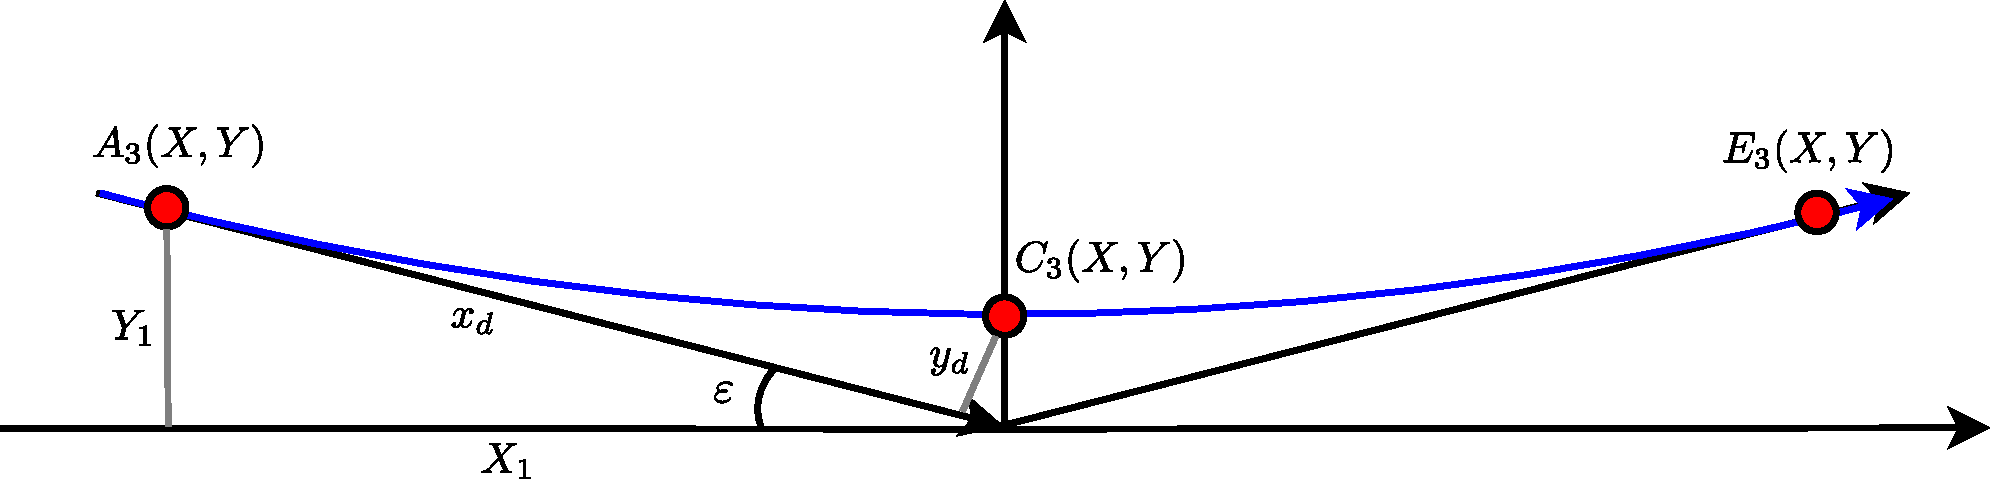
\includegraphics[width=8.4cm]{img/3Points} % width of a column is 8.4 cm.
		\caption{Path planning when $\varepsilon$ < $\varepsilon_{max}$, the path is composed by two identical but mirrored Euler-spirals. 3 key points are generated, denoted $A_3$, $C_3$ and $E_3$}
		\label{fig:3points}
	\end{center}
\end{figure}
The 3 key points are given by the coordinate sets:
\begin{align}
A_3 = (-X_1,Y_1),\, C_3 = (0,\frac{y_d}{cos(\varepsilon)}),\, E_3 = (X_1,Y_1)
\end{align}
From where the individual coordinates can be computed by simple trigonometric equations, if the angle of the turn $\varepsilon$ is known. $x_d$ and $y_d$ are the length of the scaled Euler-spiral, when the turn of the spiral equals to $\varepsilon$, where $x_d$ and $y_d$ represents the $(x,y)$ coordinate pair of the two normalized Fresnel integral functions with the same parameter $t$. 
\begin{align}
\varepsilon = \frac{\textrm{dx }F(t)}{\textrm{dy}} \quad \to \quad [x_d,y_d] = F^{-1}(\varepsilon)
\end{align}
Once the angle grows larger than $\varepsilon_{max}$ the system has to compute five key points, as the ship must transit onto a curve, and then back onto the Euler spiral ($\kappa_{Euler_{max}} = \kappa_{Arc}$) This adds the extra waypoints $B_5$ and $D_5$, the entry and exit points of the curve. The center of the circular path segment is $O_5$ and the radius is $R_{min} = \frac{1}{\kappa_{max}}$. The waypoints are depicted on figure (\ref{fig:5points}), which augments the waypoint calculations to:
\begin{figure}
	\begin{center}
		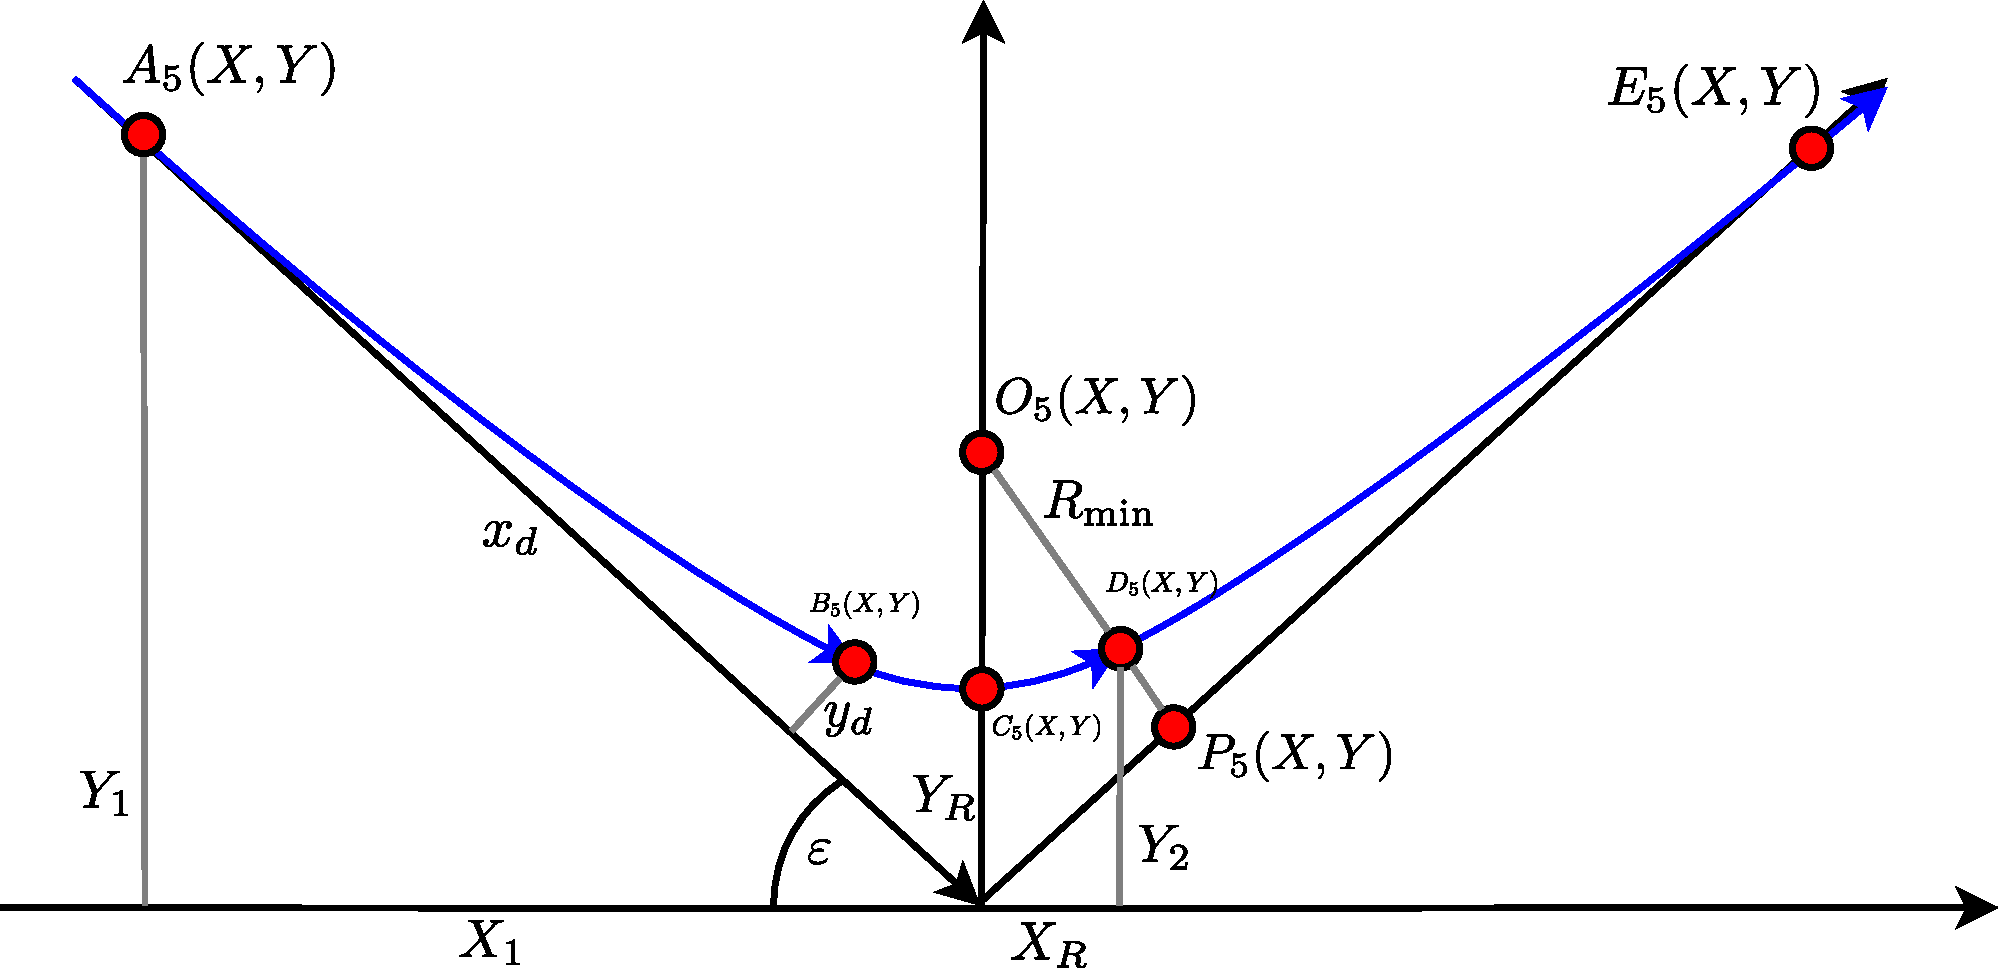
\includegraphics[width=8.4cm]{img/5Points}    % The printed column  
		\caption{Path planning when $\varepsilon$ < $\varepsilon_{max}$, the path is approximated by a curve and 5 key points are generated, denoted $A_5$, $B_5$, $C_5$, $D_5$ and $E_5$}  % width of a column is 8.4 cm.
		\label{fig:3points}               
	\end{center}                                 % accordingly.
\end{figure}
\begin{align}
A_5 &= (-X_1,Y_1),\, B_5 = (-X_2,Y_2),\, C_5 = (0,Y_R)\\
D_5 &= (X_2,Y_2),\, E_5 = (X_1,Y_1)
\end{align}
Which is still a mirroring of points about the $x=0$ axis, as the entry angle is the same as the exit angle. The number of equations increases, and the individual coordinates can be computed by:
\begin{align}
X_R &= R_\text{min} \cdot \sin(\varepsilon - \varepsilon _\text{max}),\,\, P_X = X_R + y_d \cdot \sin(\varepsilon)\\
X_1 &= P_X + x_d \cdot \cos(\varepsilon),\,\, Y_1 = X_1 \cdot \tan(\varepsilon)\\
P_Y &= Y_1 - x_d \cdot \sin(\varepsilon),\,\, Y_2 = P_Y + y_d \cdot \cos(\varepsilon)\\
O_Y &= R_\text{min} \cdot \cos(\varepsilon - \varepsilon _\text{max}) + Y_2,\,\, Y_R = O_Y - R_\text{min}\\
X_2 &= X_R
\end{align}

The resulting path in both cases can not be described explicitly, therefore a Hermite-polynom is fit to the key points. In addition, a predefined number of uniformly distributed sub-waypoints are generated on the path, based on the describing polynom. The resulting sub-waypoints are rotated and moved to their correct position in the Local-Frame, thus concluding most of the work of the local-planner. The paths between turns are straight lines, populated with the same preset density of sub-waypoints.

\subsection{Navigation}

The navigation controller of the ship is a general reference heading calculator, which outputs the required direction of movement to reach the next waypoint. In order to efficiently and accurately navigate along the path, a set of Sub-Waypoints is calculated for each route between two Waypoints. The main control strategy is to navigate through all of these SWPs in a predefined order, one by one. The heading of the ship is defined in NED\footnote[1]{[North, East, Down]} coordinate system. The required heading is determined based on the Position of the Ship and the Position of the next sub-waypoint.

\subsection{State estimation}
To give a better estimate of position and the attitude of the craft, a Kalman filter have been implemented to improve the accuracy of the sensors mounted aboard the ship. To develop a such, the discrete time state model of the ship have been derived to be:
\begin{align}
\vec{\Phi} = diag\{\vec{\Phi} _x,\vec{\Phi} _y,\vec{\Phi} _\omega\}
\end{align}
Where the diagonal entries $\vec{\Phi} _x,\vec{\Phi} _y,\vec{\Phi} _\omega$ are given by the same equation, with different entries:
\begin{align}
\vec{\Phi}_{x,y,\omega}(k) = \begin{bmatrix}
1 & t_s & 0\\
0 & 1 & t_s\\
0 & -\beta_{x,y,\omega} & 0
\end{bmatrix}
\label{eq:kal}
\end{align}
In equation (\ref{eq:kal}), $\beta_{x,y,\omega}$ denotes the skin frictional acceleration drag in the $x$,$y$ and $\omega$ direction respectively, $m$ is the mass of the craft, $I$ is the inertia and $t_s$ is the sampling time of the filter. The states to be estimated for the controller are:
\begin{align}
^b\hat{\vec{x}_k} = \begin{bmatrix}
x & \dot{x} & y & \dot{y} & \theta & \omega
\end{bmatrix}^T
\end{align}
The observation model of the filter does however contain more measurements, and the measurements can be given as:
\begin{align}
\vec{v}_k = \begin{bmatrix}
x & \dot{x} & \ddot{x} & y & \dot{y} & \ddot{y} & \theta & \omega & \alpha
\end{bmatrix}^T
\end{align}
To tune the filter the covariance matrices $\vec{R}_k$ and $\vec{Q}_k$ are a function of the measurement distribution and the input distribution. The input to the system is given as:
\begin{align}
\vec{w}_k = \vec{B}\vec{u}
\end{align}
Where $\vec{B}$ is an augmented version of the system input matrix defined in INSERT REFERENCE! and $\vec{u}$ is the inputs to the system given as a force $F$ and a torque $\tau$. $\vec{B}$ is given as 
\begin{align}
\vec{B} = \begin{bmatrix}
0 & 0 & \frac{1}{m} & 0 & 0 & 0 & 0 & 0 & 0\\
0 & 0 & 0 & 0 & 0 & 0 & 0 & 0 & \frac{1}{I} \end{bmatrix}^T
\end{align} 
And the input is given as $\vec{u} = \begin{bmatrix}F\ & \tau\end{bmatrix}^T$. As $\vec{B}$ is a static matrix, it is only the distribution of the force $F$ and the torque $\tau$ that is of interest. The distribution of the force are split into an $x$-component and a $y$-component, as the ship is also expected to move in the $y$-direction. The distributions of the force is givne as white Guassian noise processes, thus stating:
\begin{align}
F&\sim \mathcal{N}(\vec{\mu}_F,\vec{\sigma}^2_F)\\
\tau&\sim \mathcal{N}(\mu_\tau,\sigma^2_\tau)
\end{align}
Where the tuning through simulations have yielded the best results using $\vec{\mu}_F = \begin{bmatrix}5.4355 & 0\end{bmatrix}^T$. The first entry is because to the ship is for most of the time moving along at 1 m/s and that is the estimated force required to thrust the ship forward at 1 m/s with the frictional drag the ship experiences. The latter is the force in the $y$-direction which is given as a zero-mean process as the ship is not expected to move sideways. The torque is also given as a zero-mean process as the ship for most of the time is moving straight. The covariance matrix for the input, can thus be given as the covariance of $\vec{B}\vec{u}$ which gives the following:
\begin{align}
\vec{R}_k = \text{diag}\{0,0,\sigma^2_{F(1,1)},0,0,\sigma^2_{F(2,1)},0,0,\sigma^2_\tau\}
\end{align}
The measurement covariance is more interesting, as this contains the actual variance of the measurements, and play a big part in how much each of these are weighted in Kalman gain $\bar{\vec{K}}$. Static tests have been conducted to estimate these variances, and all the sensors are assumed to be Gaussian white noise processes, thus defining:
\begin{align}
\vec{v}_k  \sim \mathcal{N}(\vec{\mu}_v,\vec{\sigma}^2_{v})
\end{align}
As all the measurements are independent, the covariance matrix is given as:
\begin{align}
\vec{Q}_k = \text{diag}\{\vec{\sigma}^2_{v}\}
\end{align}
Where $\vec{\sigma}^2_{v} = \begin{bmatrix}\sigma^2_x & \sigma^2_{\dot{x}} & \sigma^2_{{\ddot{x}}} & \sigma^2_y & \sigma^2_{\dot{y}} & \sigma^2_{{\ddot{y}}} & \sigma^2_\theta & \sigma^2_\omega & \sigma^2_\alpha \end{bmatrix}^T$. As the velocity output of the GPS device $\dot{x}$ is an absolute value, the estimate of this is a bit different as this cannot be assumed to be a normal distribution, as it does not contain any negative values. To estimate the variance of $\dot{x}$ the unbiased sample variance formula is used, which computes the variance, even though the samples only consist of absolute values. 

The actual implementation of the filter is an altered version of an Linear Minimum Mean Square Error filter - the alteration lies in the Kalman gain, where a matrix mask $\vec{\Lambda}$ is post multiplied. This matrix mask is to zero out the measurements that are invalid. This matrix mask is defined as:
\begin{align}
\vec{\Lambda} = diag\{ \lambda_x,\lambda_{\dot{x}},\lambda_{\ddot{x}},\lambda_y,\lambda_{\dot{y}},\lambda_{\ddot{y}},\lambda_{\theta},\lambda_{\omega},\lambda_{\alpha} \}
\end{align}
This ensures that when a measurement is invalid (the checksum is not true) the receiver zeros out the gain, and runs the filter on the other sensors / estimates. The individual $\lambda$s are thus given as:
\begin{align}
\lambda = 
\left\{
  \begin{array}{l l}
    1 & \quad \text{if checksum is valid}\\
    0 & \quad \text{otherwise}
  \end{array} \right.
\end{align} 
This makes sure to zero out the Kalman gain $\bar{\vec{K}}$ if a packet is corrupted instead of making the filter run on faulty data. When this is implemented, the system handles not present measurements by making the filter run on estimates for the next sample, rather than running on a faulty measurement.

\subsection{Modelling and Controls}
The model of the ASV is in continuos time given as the state space equation defined in (eq:\ref{eq:ss_cont}) - the model considers the motion of the ship with 3 degrees of freedom, movement in the $x$-direction, $y$-direction and rotation about the z-axis $\omega$. 
\begin{align}
\dot{\begin{bmatrix}
v\\
\theta\\
\omega
\end{bmatrix}} = \begin{bmatrix}
-\beta_v & 0 & 0\\
0 & 0 & 1\\
0 & 0 & -\beta_\omega
\end{bmatrix} \begin{bmatrix}
v\\
\theta\\
\omega
\end{bmatrix} + \begin{bmatrix}
m^{-1} & 0\\
0 & 0\\
0 & I^{-1}
\end{bmatrix}\begin{bmatrix}
F\\
\tau
\end{bmatrix}
\label{eq:ss_cont}
\end{align}
Where $\beta_{v,\omega}$ is the acceleration drag experienced by the ship in the $x$-direction. This reduced model is sufficient as it is only the velocity and the angle that is control variables. The control strategy for this project is to track the input reference, and use an optimal feedback gain to reach the desired values. This is done as in \cite{feedback} resulting in the following gains:
\begin{align}
F_{opt} &= \begin{bmatrix}
15.1668 & 0 & 0\\
0 & 2.5165 & 0.7134
\end{bmatrix}\label{eq:fcont}\\
N &=  \begin{bmatrix}
24.0668 & 0\\
0 & 2.5165
\end{bmatrix}\label{eq:ncont}
\end{align}
For implementation purposes the system is discretized using the MATLAB command \texttt{c2d} with a samping time of $t_s = \frac{1}{3}$, and then using the same algorithms as in equation (\ref{eq:fcont}) and (\ref{eq:ncont}) for computing the optimal feedback and reference gain respectively, thus resulting in the gains (\ref{eq:fdisc}) and (\ref{eq:ndisc}):
\begin{align}
_\mathcal{D}F_{opt} &= \begin{bmatrix}
10.6956 & 0 & 0\\
0 & 2.2743 & 0.6681
\end{bmatrix}\label{eq:fdisc}\\
_\mathcal{D}N &=  \begin{bmatrix}
19.5956 & 0\\
0 & 2.2743
\end{bmatrix}\label{eq:ndisc}
\end{align}
As the controller outputs a desired force $F$ and a torque $\tau$ dependent on the reference angle $\theta$ and velocity $\theta$. This output must be converted to a set-point number of revolutions, as this is the input to the low-level system handling the engines. The force of the forward motion of the ship is given as a function of the number of revolutions of the propeller $n$, this relation is defined by \cite{cyber} to be:
\begin{align}
F_1 &= C_1 \cdot \text{abs}\{n_1\} \cdot n_1\\
F_2 &= C_1 \cdot \text{abs}\{n_2\} \cdot n_2
\end{align}
Where $C_1 = \rho \cdot K_T \cdot D^4$, which are constant for both the engines. The two propellers thus produce a total force as a sum of these functions. The torque produced by the propellers can be described as $F$ multiplied with the distance to the propeller.
\begin{align}
\tau_1 &= F_1 \cdot \sin(\theta_\text{stbd.engine})\\
\tau_2 &= F_2 \cdot \sin(\theta_\text{port.engine})
\end{align}
As the two engines both produce a force and a torque, as a function of the same revolutions, the matrix equation $\vec{x} = \vec{A}^{-1}\vec{b}$ can be solved for the number of revolutions the engines need to produce as in (\ref{eq:solver}):
\begin{align}
\begin{bmatrix}
n_1^2\\
n_2^2
\end{bmatrix} = \begin{bmatrix}
C_1 & C_1\\
C_1 \cdot \sin(\theta) & C_1 \cdot \sin(-\theta)
\end{bmatrix}^{-1}\begin{bmatrix}
F_\text{desired}\\
\tau_\text{desired}
\end{bmatrix}\label{eq:solver}
\end{align}
Whats left to do is to solve for $n_1$ and $n_2$. These can be solved by:
\begin{align}
n_1 = \frac{n_1}{\text{abs}\{n_1\}} \cdot \sqrt{\text{abs}\{n_1\}}\\
n_2 = \frac{n_2}{\text{abs}\{n_2\}} \cdot \sqrt{\text{abs}\{n_2\}}
\end{align}
Thus giving the engine set-points as a function of the force of the system. The first term $\frac{n_1}{\text{abs}\{n_1\}}$ gives the sign of the engine input, wether this should be negative or positive is defined here. The last term computes the actual revolution to be sent. 


\subsection{Controller verification}
Running the system with just the controllers produces the following plot trying to follow a path around the parking lot. 
\begin{figure}
	\begin{center}
		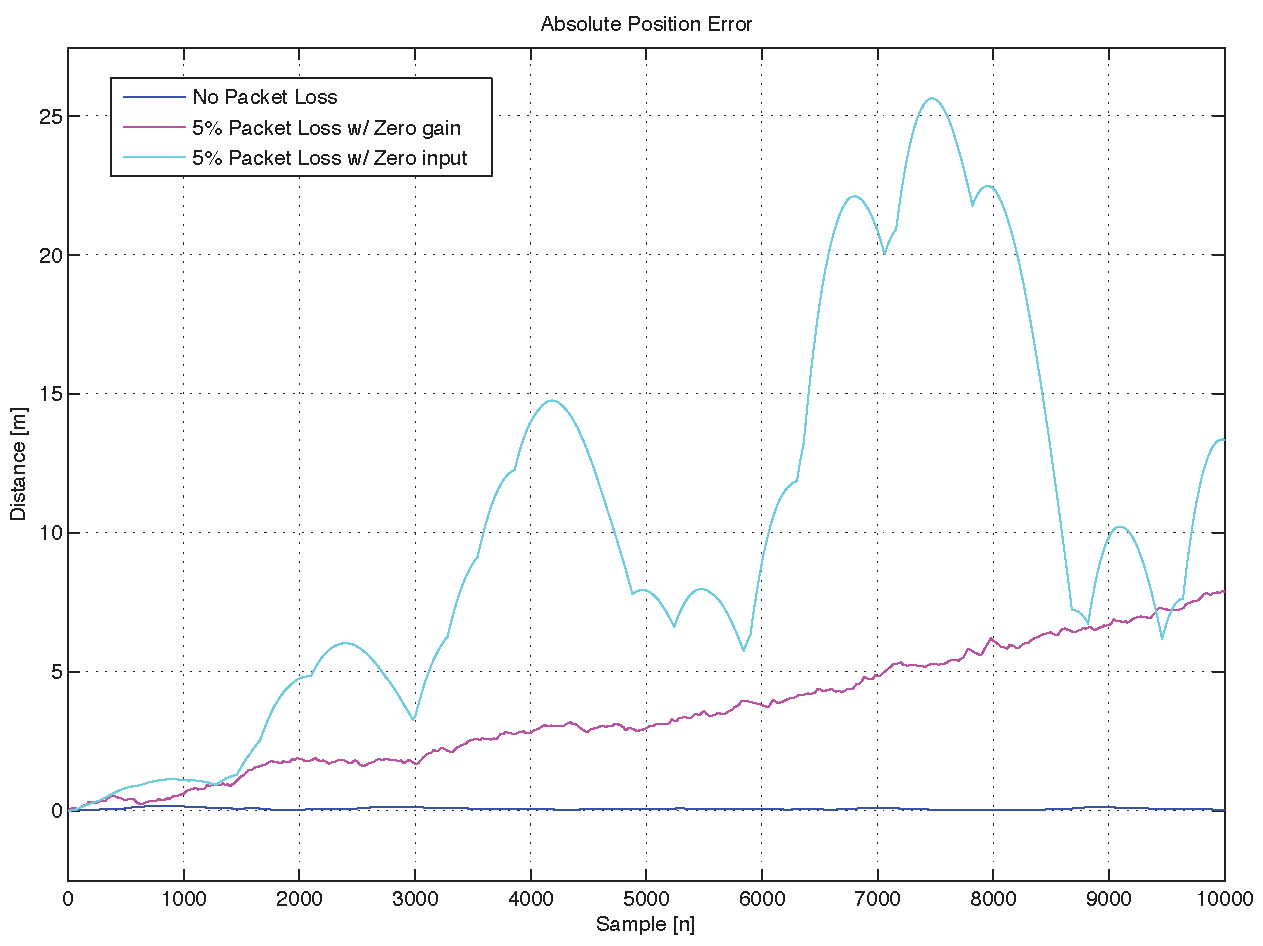
\includegraphics[width=8.4cm]{img/abspos}    % The printed column  
		\caption{CONTROLLER VERIFICATION}  % width of a column is 8.4 cm.
		\label{fig:3points}               
	\end{center}                                 % accordingly.
\end{figure}

\subsection{Path planning results}
Planning the path on a stretch of water in Aalborg produces the following results:
\begin{figure}
	\begin{center}
		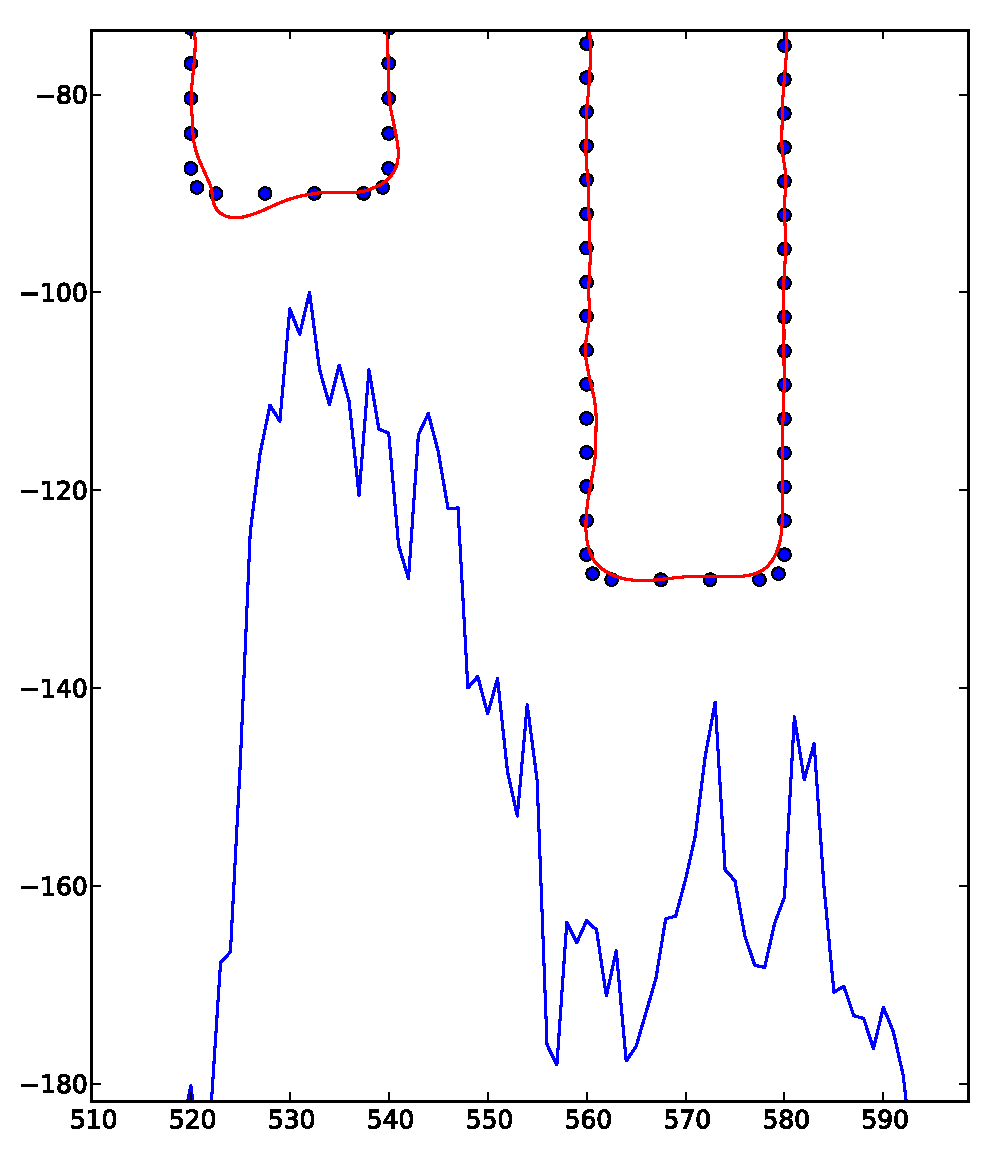
\includegraphics[width=8.4cm]{img/Navi}    % The printed column  
		\caption{Part of the simulated path of the embedded system close to the shore along the sub-waypoints, during a regular oceanography task, based on GPS position measurements affected by white noise with 4m variance. The shoreline is generated by a random walk.}  % width of a column is 8.4 cm.
		\label{fig:navi}               
	\end{center}                                 % accordingly.
\end{figure}

\subsection{Kalman filtering verification}
Filtering the above traced controller route with the Kalman filter, having the input to the system to zero, and post processing the data produces the following plot.
\begin{figure}
	\begin{center}
		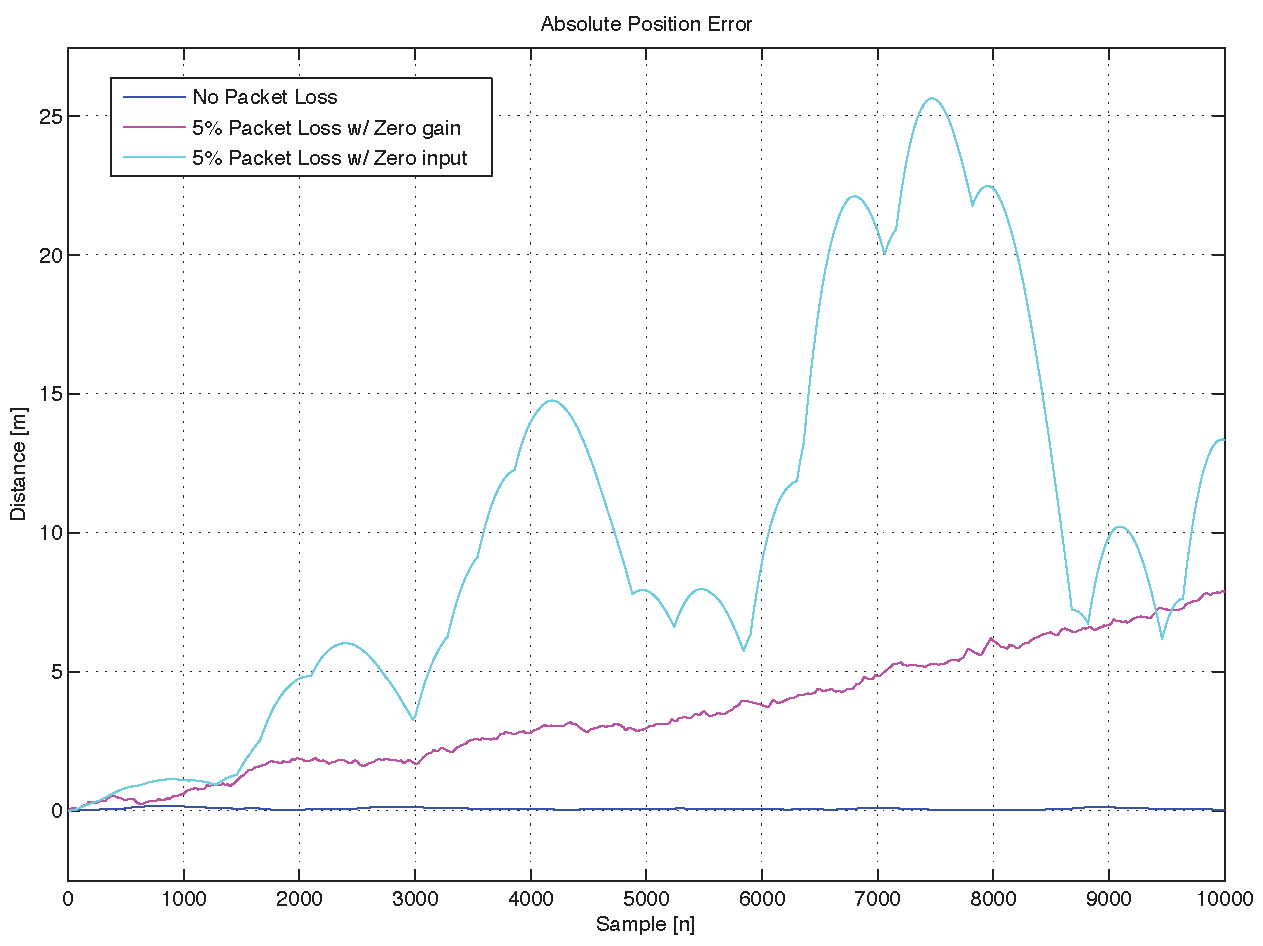
\includegraphics[width=8.4cm]{img/abspos}    % The printed column  
		\caption{KALMAN FILTERING VERIFICATION}  % width of a column is 8.4 cm.
		\label{fig:3points}               
	\end{center}                                 % accordingly.
\end{figure}

\subsection{Combined test}
Running the Kalman filter on the ship whilst in motion. As seen some packages are lost - to verify the simulator, a simulation have been run with the same amount of packages lost, and this produces the same result. 
\begin{figure}
	\begin{center}
		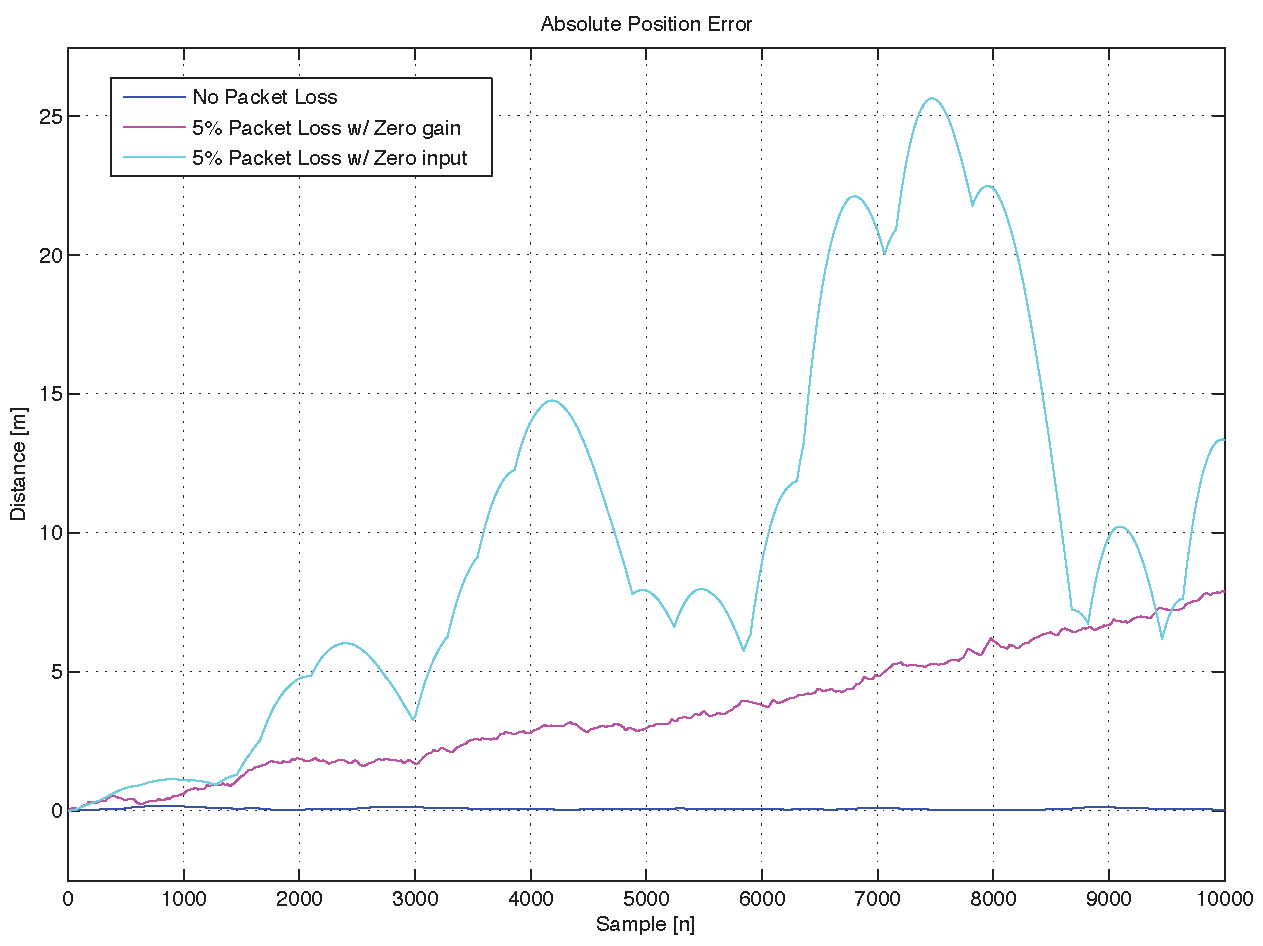
\includegraphics[width=8.4cm]{img/abspos}    % The printed column  
		\caption{COMBINED TEST}  % width of a column is 8.4 cm.
		\label{fig:3points}               
	\end{center}                                 % accordingly.
\end{figure}

Something about the packet loss. 

\subsection{Discussion}

As the above results have given an error 


\section{Conclusion}
To sum up the project, a state estimator have been developed to improve on the GPS estimates. Such an estimator have been developed, and it have been seen that the estimates are better than what the GPS measures, and the box is able to give a better estimate 

\begin{ack}                               % Place acknowledgements
A special thank should be given to Assistant Professor Carles Navarro Manchòn, Section for Navigation and Communication, Department of Electronic Systems, Aalborg University for his help with tuning the Kalman filter.  % here.
\end{ack}

%\bibliographystyle{alpha}        % Include this if you use bibtex 
%\bibliography{autosam}           % and a bib file to produce the 
%\bibliography{autosam}
                                 % bibliography (preferred). The
                                 % correct style is generated by
                                 % Elsevier at the time of printing.

\begin{thebibliography}{xx}

\bibitem[Ingeni\o ren(2012)]{engineer}
Birgitte Marfelt,
\newblock Ingeni\o ren
\newblock \emph{Tom pengekasse bremser søkort omkring Gr\o nland}
\newblock Mediehuset Ingeniøren, 2012

\bibitem[Talbot(1901)]{Art:1}
Arthur N. Talbot,
\newblock \emph{The Railway Transition Spiral}
\newblock The Engeneering News Publishing Co., 1901

\bibitem[K\'oml\'osi-Kiss(2011)]{Art:2} % The name shown in the report, and the lable \cite{Art:1}
Istv\'a n Koml\'{o}si \& B\'a lint Kiss, % Name of the author
\newblock \emph{Mobilis robotok auton\'{o}m navig\'aci\'{o}ja mozg\'{o} akad\'alyok elker\"ul\'es\'evel} % The name of the thesis
\newblock Budapest University of Technology and Economics, 2011 % The publisher

\bibitem[S\o rensen(2005)]{cyber}
Asgeir J. S\o rensen,
\newblock \emph{Marine Cybernetics, Modelling and Control - Lecture Notes}
\newblock Department of Marine Cybernetics, Norwegian University of Science and Technology, 2005

\bibitem[Franklin et. al.(2009)]{feedback}
Gene F. Franklin, J. David Powell and Abbas Emami-Naeini,
\newblock \emph{Feedback Control of Dynamic Systems, 5th ed.}
\newblock Pearson Prentice Hall, 2009

\end{thebibliography}








\appendix
\section{A summary of Latin grammar}    % Each appendix must have a short title.
\section{Some Latin vocabulary}         % Sections and subsections are supported  
                                        % in the appendices.
\end{document}
